% Copyright 2004 by Till Tantau <tantau@users.sourceforge.net>.
%
% In principle, this file can be redistributed and/or modified under
% the terms of the GNU Public License, version 2.
%
% However, this file is supposed to be a template to be modified
% for your own needs. For this reason, if you use this file as a
% template and not specifically distribute it as part of a another
% package/program, I grant the extra permission to freely copy and
% modify this file as you see fit and even to delete this copyright
% notice. 

\documentclass{beamer}

\usepackage{kotex}
\usepackage{graphicx,psfrag,amsfonts,amsmath,amssymb}
\usepackage{multicol}

% There are many different themes available for Beamer. A comprehensive
% list with examples is given here:
% http://deic.uab.es/~iblanes/beamer_gallery/index_by_theme.html
% You can uncomment the themes below if you would like to use a different
% one:
%\usetheme{Dresden}
%\usetheme{AnnArbor}
%\usetheme{Antibes}
%\usetheme{Bergen}
%\usetheme{Berkeley}
\usetheme{Berlin}
%\usetheme{Boadilla}
%\usetheme{boxes}
%\usetheme{CambridgeUS}
%\usetheme{Copenhagen}
%\usetheme{Darmstadt}
%\usetheme{default}
%\usetheme{Frankfurt}
%\usetheme{Goettingen}
%\usetheme{Hannover}
%\usetheme{Ilmenau}
%\usetheme{JuanLesPins}
%\usetheme{Luebeck}
%\usetheme{Madrid}
%\usetheme{Malmoe}
%\usetheme{Marburg}
%\usetheme{Montpellier}
%\usetheme{PaloAlto}
%\usetheme{Pittsburgh}
%\usetheme{Rochester}
%\usetheme{Singapore}
%\usetheme{Szeged}
%\usetheme{Warsaw}

\usecolortheme{lily}
\usefonttheme[onlymath]{serif}	% 수식 설정!!

\title{Functional Data Analysis}
%\date{\today}
\date[Short Occasion]{April 26, 2019}
\author{Hyunsung Kim}
\institute[Yaeji Lim's Lab]
	{Department of Statistics\\
	Chung-Ang University}

% A subtitle is optional and this may be deleted
\subtitle{Tools for exploring functional data and Functional PCA}

%\author{F.~Author\inst{1} \and S.~Another\inst{2}}
% - Give the names in the same order as the appear in the paper.
% - Use the \inst{?} command only if the authors have different
%   affiliation.

%\institute[Universities of Somewhere and Elsewhere] % (optional, but mostly needed)
%{
%  \inst{1}%
%  Department of Computer Science\\
%  University of Somewhere
%  \and
%  \inst{2}%
%  Department of Theoretical Philosophy\\
%  University of Elsewhere}
% - Use the \inst command only if there are several affiliations.
% - Keep it simple, no one is interested in your street address.

%\date{Conference Name, 2013}
% - Either use conference name or its abbreviation.
% - Not really informative to the audience, more for people (including
%   yourself) who are reading the slides online

\subject{Functional Data Analysis}
% This is only inserted into the PDF information catalog. Can be left
% out. 

% If you have a file called "university-logo-filename.xxx", where xxx
% is a graphic format that can be processed by latex or pdflatex,
% resp., then you can add a logo as follows:

% \pgfdeclareimage[height=0.5cm]{university-logo}{university-logo-filename}
% \logo{\pgfuseimage{university-logo}}

% Delete this, if you do not want the table of contents to pop up at
% the beginning of each subsection:
\AtBeginSubsection[]
{
  \begin{frame}<beamer>{Outline}
    \tableofcontents[currentsection,currentsubsection]
  \end{frame}
}

% Let's get started
\begin{document}

\begin{frame}
  \titlepage
\end{frame}

\begin{frame}{Outline}
  \tableofcontents
  % You might wish to add the option [pausesections]
\end{frame}

% Section and subsections will appear in the presentation overview
% and table of contents.
\section{Tools for exploring functional data}

\subsection{Introduction}

\begin{frame}{Introduction}
  \begin{itemize}
  	\item {
	    FDA의 notation과 concept 정의
	}
	\item {
		FDA에서 사용하는 statistics 정의
	}
	\item {
		Matrix decompositions, projections, and the constrained maximization of quadratic forms에 대한 자세한 내용은 Appendix 참고
	}
  \end{itemize}
\end{frame}

\subsection{Some notation}

% You can reveal the parts of a slide one at a time
% with the \pause command:
\begin{frame}{Scalars, vectors, functions and matrices}
  \begin{itemize}
	\item {
		$x$ : a vector \\
		$\Rightarrow x_i$ : scalar (the elements of vector $x$)
	}
	\item {
		$x$ : a function \\
		$\Rightarrow x(t)$ : scalar (the values of function $x$) \\
		$\Rightarrow x(\mathbf{t})$ : vector $\mathbf{t}$에 대한 function value ($p$-dim function)
	}
	\item {
		If $x_i$ or $x(t)$ is a vector, we use $\boldsymbol{x}_i$ or $\boldsymbol{x}(t)$
	}
	\item {
		Standard notation을 요약하여 사용
	    \begin{itemize}
			\item
				\texttt{Temp} : a temperature record
			\item
				\texttt{Knee} : a knee angle
			\item
				\texttt{LMSSE} : a squared error fitting criterion for a linear model
			\item
				\texttt{RSQ} : a squared correlation measure.
		\end{itemize}	
	}
  \end{itemize}
\end{frame}

\begin{frame}{Derivatives and integrals}
	\begin{itemize}
		\item {
			$D$ : $operator$ (함수 $x$를 함수 $Dx$로 변환하는 $operator$)
		}
		\item {
			$D^m x$ : the derivative of order m of a function $x$ ($\frac{d^mx}{dt^m}$와 동일)
		}
		\item {
			$D^0 x$ : $x$ \\
			$s.t. \ D^{1}D^{-1}x=D^0x=x$,\\
			when $D^{-1}x$가 $x$의 부정적분(indefinite integral)
		}
		\item {
			$\int x$ : $\int_{a}^{b} x(t)dt$ \ ($t$의 적분 범위가 clear할 때)
		}
	\end{itemize}
\end{frame}

\begin{frame}{Inner products}
	\begin{itemize}
		\item {
			Inner product for functions\\
			$$\langle x,y \rangle = \int x(t)y(t)dt $$
		}
		\item {
			$L_2$ norm \\
			$$ \lVert x \rVert^2=\langle x,x \rangle = \int x^2(t)dt $$
		}
	\end{itemize}
\end{frame}

\begin{frame}{Functions of functions}
	\begin{itemize}
		\item {
			functional composition (합성함수) \\
			$$ x^*=x \circ h $$	
		}
		\item {
			function value \\
			$$ x^*(t)=(x \circ h)(t)=x[h(t)] $$
		}
		\item {
			inverse function $h^{-1}$\\
			$$ (h \circ h^{-1})(t)=(h^{-1} \circ h)(t)=t $$
		}	
		\item {
			functional transformations $operations$ (or $operators$) \\
			ex) $D$ : $x \rightarrow Dx$
		}	
	\end{itemize}
\end{frame}


\subsection{Summary statistics for functional data}

% You can reveal the parts of a slide one at a time
% with the \pause command:
\begin{frame}{Functional means and variances}
  \begin{itemize}
	\item {
		Mean function
		$$ \bar{x}(t)=\frac{1}{N}\sum_{i=1}^{N}x_i(t) $$
	}
	\item {
		Variance function
		$$ Var_X(t)=\frac{1}{N-1}\sum_{i=1}^{N}[x_i(t)-\bar{x}(t)]^2 $$
	}
  \end{itemize}
\end{frame}

\begin{frame}{Functional means and variances}
\begin{figure}[h] %%% t: top, b: bottom, h: here
	\begin{center}
		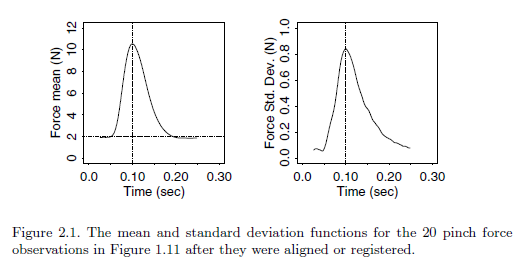
\includegraphics[width=1\linewidth]{img/1.png}
	\end{center}
	%\caption{Sampling two normal mixture(histogram) VS True normal mixture(red line)}
	\label{fig:long}
	\label{fig:onecol}
\end{figure}	
%\begin{itemize}
%	\item {
%		figure 설명
%	}
%\end{itemize}
\end{frame}

\begin{frame}{Covariance and correlation functions}
	\begin{itemize}
		\item {
			Covariance function
			$$ Cov_X(t_1, t_2)=\frac{1}{N-1}\sum_{i=1}^{N}\{x_i(t_1)-\bar{x}(t_1)\}\{x_i(t_2)-\bar{x}(t_2)\} $$
		}
		\item {
			Correlation function
			$$ Corr_X(t_1, t_2)=\frac{Cov_X(t_1, t_2)}{\sqrt{Var_X(t_1)Var_X(t_2)}} $$
		}
	\end{itemize}
\end{frame}

\begin{frame}{Covariance and correlation functions}
	\begin{figure}[h] %%% t: top, b: bottom, h: here
		\begin{center}
			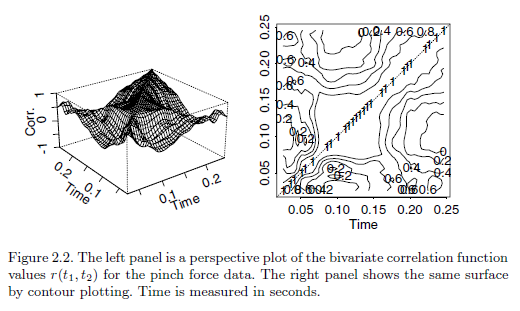
\includegraphics[width=1\linewidth]{img/2.png}
		\end{center}
		%\caption{Sampling two normal mixture(histogram) VS True normal mixture(red line)}
		\label{fig:long}
		\label{fig:onecol}
	\end{figure}	
%	\begin{itemize}
%		\item {
%		figure 설명
%		}
%	\end{itemize}
\end{frame}

\begin{frame}{Cross-covariance and cross-correlation functions}
	\begin{itemize}
		\item {
			Cross-covariance function
			$$ Cov_{X,Y}(t_1, t_2)=\frac{1}{N-1}\sum_{i=1}^{N}\{x_i(t_1)-\bar{x}(t_1)\}\{y_i(t_2)-\bar{y}(t_2)\} $$
		}
		\item {
			Cross-correlation function
			$$ Corr_{X,Y}(t_1, t_2)=\frac{Cov_{X,Y}(t_1, t_2)}{\sqrt{Var_X(t_1)Var_Y(t_2)}} $$
		}
	\end{itemize}
\end{frame}

\begin{frame}{Cross-covariance and cross-correlation functions}
	\begin{figure}[h] %%% t: top, b: bottom, h: here
		\begin{center}
			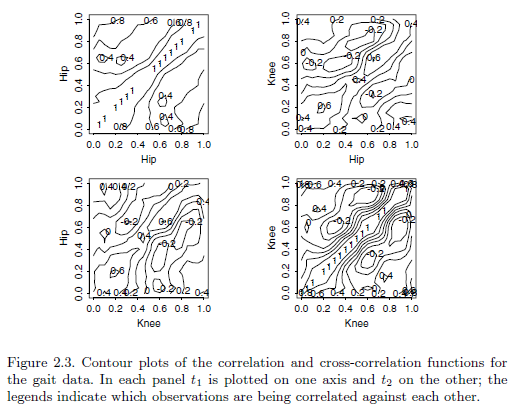
\includegraphics[width=0.75\linewidth]{img/3.png}
		\end{center}
		%\caption{Sampling two normal mixture(histogram) VS True normal mixture(red line)}
		\label{fig:long}
		\label{fig:onecol}
	\end{figure}
%	\begin{itemize}
%		\item {
%			Figure 설명
%		}
%	\end{itemize}
\end{frame}

\begin{frame}{Cross-covariance and cross-correlation functions}{Cantour plots of correlation functions}
	\begin{multicols}{2}
		\begin{figure}[h] %%% t: top, b: bottom, h: here
			\begin{center}
				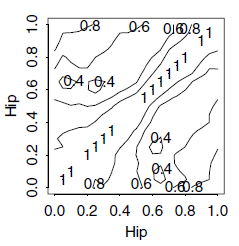
\includegraphics[width=0.9\linewidth]{img/6.png}
			\end{center}
			%\caption{Sampling two normal mixture(histogram) VS True normal mixture(red line)}
			\label{fig:long}
			\label{fig:onecol}
		\end{figure}
		\begin{figure}[h] %%% t: top, b: bottom, h: here
			\begin{center}
				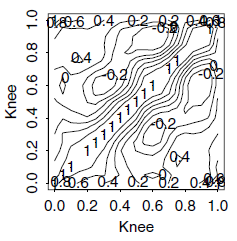
\includegraphics[width=0.9\linewidth]{img/7.png}
			\end{center}
			%\caption{Sampling two normal mixture(histogram) VS True normal mixture(red line)}
			\label{fig:long}
			\label{fig:onecol}
		\end{figure}
	\end{multicols}
\end{frame}

\begin{frame}{Cross-covariance and cross-correlation functions}{Cantour plots of cross-correlation functions}
\begin{multicols}{2}
	\begin{figure}[h] %%% t: top, b: bottom, h: here
		\begin{center}
			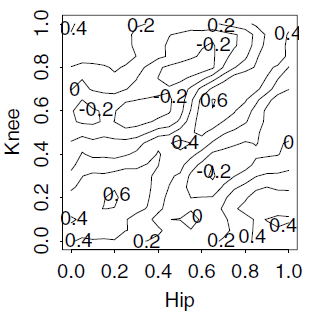
\includegraphics[width=0.9\linewidth]{img/8.png}
		\end{center}
		%\caption{Sampling two normal mixture(histogram) VS True normal mixture(red line)}
		\label{fig:long}
		\label{fig:onecol}
	\end{figure}
	\begin{figure}[h] %%% t: top, b: bottom, h: here
		\begin{center}
			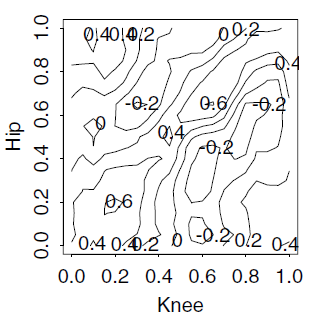
\includegraphics[width=0.9\linewidth]{img/9.png}
		\end{center}
		%\caption{Sampling two normal mixture(histogram) VS True normal mixture(red line)}
		\label{fig:long}
		\label{fig:onecol}
	\end{figure}
\end{multicols}
\end{frame}


\begin{frame}{Cross-covariance and cross-correlation functions}
\begin{figure}[h] %%% t: top, b: bottom, h: here
	\begin{center}
		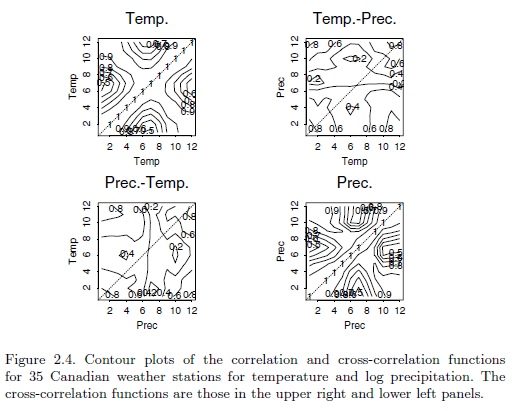
\includegraphics[width=0.75\linewidth]{img/4.png}
	\end{center}
	%\caption{Sampling two normal mixture(histogram) VS True normal mixture(red line)}
	\label{fig:long}
	\label{fig:onecol}
\end{figure}
%\begin{itemize}
%	\item {
%		Figure 설명
%	}
%\end{itemize}
\end{frame}

\begin{frame}{Cross-covariance and cross-correlation functions}{Cantour plots of correlation functions}
\begin{multicols}{2}
	\begin{figure}[h] %%% t: top, b: bottom, h: here
		\begin{center}
			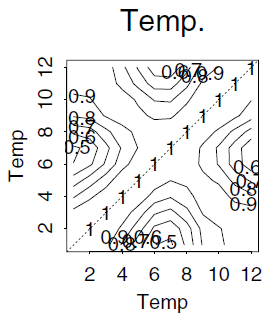
\includegraphics[width=0.9\linewidth]{img/10.png}
		\end{center}
		%\caption{Sampling two normal mixture(histogram) VS True normal mixture(red line)}
		\label{fig:long}
		\label{fig:onecol}
	\end{figure}
	\begin{figure}[h] %%% t: top, b: bottom, h: here
		\begin{center}
			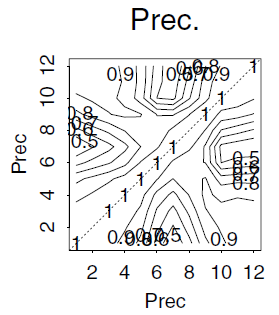
\includegraphics[width=0.9\linewidth]{img/11.png}
		\end{center}
		%\caption{Sampling two normal mixture(histogram) VS True normal mixture(red line)}
		\label{fig:long}
		\label{fig:onecol}
	\end{figure}
\end{multicols}
\end{frame}

\begin{frame}{Cross-covariance and cross-correlation functions}{Cantour plots of cross-correlation functions}
\begin{multicols}{2}
	\begin{figure}[h] %%% t: top, b: bottom, h: here
		\begin{center}
			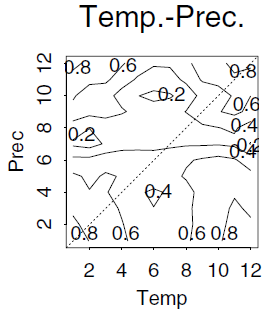
\includegraphics[width=0.9\linewidth]{img/12.png}
		\end{center}
		%\caption{Sampling two normal mixture(histogram) VS True normal mixture(red line)}
		\label{fig:long}
		\label{fig:onecol}
	\end{figure}
	\begin{figure}[h] %%% t: top, b: bottom, h: here
		\begin{center}
			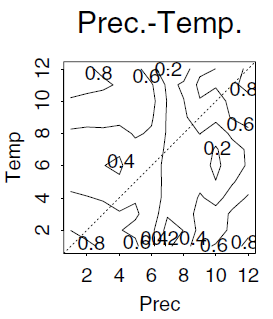
\includegraphics[width=0.9\linewidth]{img/13.png}
		\end{center}
		%\caption{Sampling two normal mixture(histogram) VS True normal mixture(red line)}
		\label{fig:long}
		\label{fig:onecol}
	\end{figure}
\end{multicols}
\end{frame}

\section{Principal components analysis for functional data}

\subsection{Introduction}

\begin{frame}{Introduction}
	\begin{itemize}
		\item {
			전처리와 시각화 후, data의 특성을 파악하기 위해 PCA를 사용
		}
		\item {
			Classical multivariate anlaysis에서는 variance-covariance와 correlation을 설명하기 힘든 경우가 많음
		}
		\item {
			PCA는 유용한 정보를 담고 있는 covariance structure를 파악하는데 도움을 준다.
		}
		\item {
			PCA를 통해 이후의 분석에서 발생할 수 있는 문제를 사전에 고려할 수 있다. (ex - multicollinearity)
		}
		\item {
			FPCA(functional PCA)는 smoothing 되어있는 경우에 특성이 더 잘 나타난다. (smoothing 과정에서 $regularization$ issue 발생)
		}
	\end{itemize}
\end{frame}

\subsection{Defining functional PCA}

\begin{frame}{PCA for multivariate data}{Concept of multivariate PCA}
	\begin{itemize}
		\item {Linear combination of X
			$$ f_i = \sum_{j=1}^{p}\beta_j x_{ij}, \ i=1,...,N $$
			where $\beta_j$ : weighting coefficient, $x_{ij}$ : $i$th obs of $j$th variable
		}
		\item {Vectorized form
			$$ f_i = \boldsymbol{\beta}^{'} \boldsymbol{x}_i, \ i=1,...,N $$
			where $ \boldsymbol{\beta}=(\beta_1,...,\beta_p)^{'}, \ \boldsymbol{x}_i=(x_{i1},...,x_{ip})^{'} $
		}
	\end{itemize}
\end{frame}

\begin{frame}{PCA for multivariate data}{How to find PC}
	\begin{itemize}
		\item {
			1. Find the weight vector $\xi_1 = (\xi_{11},...,\xi_{p1})^{'}$ for
			$$ f_{i1}=\sum_j \xi_{j1}x_{ij}=\boldsymbol{\xi}_1^{'} \boldsymbol{x}_i $$
			s.t. maximize $ \frac{1}{N}\sum_if_{i1}^2 $ subject to $\sum_j \xi_{j1}^2 = \lVert \xi_1 \rVert^2 = 1 $
		}
		\item {
			2. 1번 과정을 반복하며 동시에 
			$$ \sum_j \xi_{jk}\xi_{jm} = \boldsymbol{\xi}_k^{'} \boldsymbol{\xi}_m=0, \ k<m $$
			을 만족하는 $ \xi_2,...,\xi_m $을 찾는다.
		}
	\end{itemize}
\end{frame}

\begin{frame}{PCA for multivariate data}{Summary}
	\begin{itemize}
		\item {
			1. Mean square(변수들 간 variation)를 maximize하는 방향의 unit vector $\boldsymbol{\xi}_1 $을 찾는다.
		}
		\item {
			2. 2nd PC부터는 mean square를 maximize함과 동시에 이전 PC loading($ \boldsymbol{\xi}_i $)과 orthogonal한 $ \boldsymbol{\xi}_2,...\boldsymbol{\xi}_k \ (k<p) $을 찾는다.
		}
		\item {
			Data의 mean을 뺀 후에 PCA를 하는 것이 일반적이다. (Centering $\Rightarrow \max MS(f_{ij}) = \max Var(f_{ij}) $)
		}
		\item {
			Weight vector $\boldsymbol{\xi}_i$는 unique하지 않다. (Sign change)
		}
		\item {
			PC score $f_{im}$은 특정 사례 또는 반복실험의 특징 측면에서 변동(variation)의 의미를 설명하는데 도움을 준다.
		}
	\end{itemize}
\end{frame}

\begin{frame}{Defining PCA for functional data}{Concept of functional PCA}
\begin{itemize}
	\item {
		Inner product of integration version is defined by
		$$ \int \beta x = \int \beta(s) x(s) ds $$
	}
	\item {
		PC score
		$$ f_i = \int \beta x_i = \int \beta(s) x_i(s) ds $$
		where $\beta$ : weight function
	}
\end{itemize}
\end{frame}

\begin{frame}{Defining PCA for functional data}{How to find functional PCA}
	\begin{itemize}
		\item {
			1. Find the weight function $\xi_1(s)$ for
			$$ f_i = \int \xi_1(s) x_i(s) ds $$
			s.t. maximize $ \frac{1}{N}\sum_i f_{i1}^2 = \frac{1}{N}\sum_i (\int \xi_1 x_i)^2 $ \\
			subject to $ \lVert \xi_1 \rVert^2 =\int \xi_1(s)^2ds = \int \xi_1^2 = 1 $
		}
		\item {
			2. 1번 과정을 반복하며 동시에
			$$ \int \xi_k \xi_m=0, \ k<m $$
			을 만족하는 $ \xi_2,...,\xi_m $을 찾는다.
		}
	\end{itemize}
\end{frame}

\begin{frame}{Defining PCA for functional data}{Summary}
	\begin{itemize}
		\item {
			1. Mean square를 maximize하는 방향이고 $ \lVert \xi_1 \rVert^2=1 $인 function $\xi_1(s) $를 찾는다.
		}
		\item {
			2. 2nd PC부터는 mean square를 maximize함과 동시에 이전 PC loading($ \xi_1(s) $)와 orthogonal한 $ \xi_2(s),...\xi_k(s) \ (k<p) $을 찾는다.
		}
		\item {
			Data의 mean을 뺀 후에 PCA를 하는 것이 일반적이다. (Centering $\Rightarrow \max MS = \max Var $)
		}
		\item {
			Weight function $\xi_i(s)$는 unique하지 않다. (Sign change)
		}
	\end{itemize}
\end{frame}

\begin{frame}{Defining PCA for functional data}
	\begin{figure}[h] %%% t: top, b: bottom, h: here
		\begin{center}
			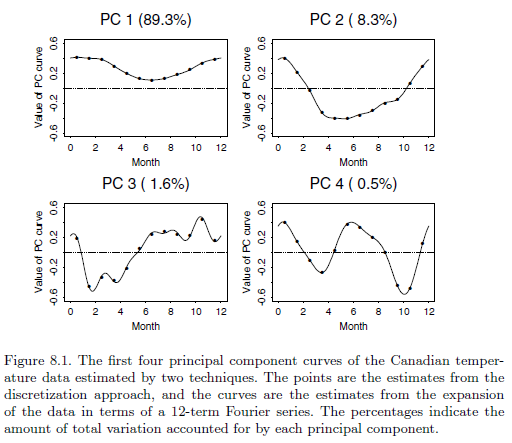
\includegraphics[width=0.7\linewidth]{img/5.png}
		\end{center}
		%\caption{Sampling two normal mixture(histogram) VS True normal mixture(red line)}
		\label{fig:long}
		\label{fig:onecol}
	\end{figure}	
\begin{itemize}
	\item {
		figure 설명
	}
	\item {
		
	}
\end{itemize}
\end{frame}

\begin{frame}{Defining an optimal empirical orthonormal basis}
\begin{itemize}
	\item {
		We want to find $K$ orthonormal functions $\xi_m$. \\
	}
	\item {
		즉, expansion했을 때 각 curve에 가장 잘 근사하는 K개의 orthonormal basis functions를 찾고 싶다!
	}
	\item {
		Expansion by the orthonormal basis functions
		$$ \hat{x}_i(t) = \sum_{k=1}^K f_{ik}\xi_{k}(t), $$
		where $ f_{ik} $ is the principal component value $\int x_i\xi_k$
	}
\end{itemize}
\end{frame}

\begin{frame}{Defining an optimal empirical orthonormal basis}
	\begin{itemize}
%		\item {
%			A fitting criterion for an individual curve
%			(Integrated squared error)
%			$$ \lVert x_i-\hat{x}_i \rVert^2=\int [x(s) - \hat{x}(s)]^2 ds $$			
%		}
		\item {
			Measure of approximation (\texttt{PCASSE})
			$$ \texttt{PCASSE} = \sum_{i=1}^N \lVert x_i-\hat{x}_i \rVert^2 $$	
			where $ \lVert x_i-\hat{x}_i \rVert^2=\int [x(s) - \hat{x}(s)]^2 ds $ (integrated squared error)	
		}
		\item {
			Optimal orthonormal basis function = weight function $\xi_m$
			$$ \xi_m = \arg\min_\xi \texttt{PCASSE} $$
			where $\xi_m$ : $empirical \ orthonormal \ functions$
		}
	\end{itemize}
\end{frame}

\begin{frame}{PCA and eigenanalysis}{Multivariate PCA}
	\begin{itemize}
		\item {
			Assumtion : $x_{ij}$ is centerized. ($x_{ij} - \frac{1}{N}\sum_i x_{ij}$)
		}
		\item {
			Mean square criterian for finding the 1st PC
			$$ \max_{\boldsymbol{\xi^{'}\xi}=1}\frac{1}{N} \boldsymbol{\xi^{'}X^{'}X\xi} $$
		}
		\item {
			Substitute variance-covariance matrix
			$$\max_{\boldsymbol{\xi^{'}\xi}=1} \boldsymbol{\xi^{'}V\xi} $$
			where $\boldsymbol{V} = N^{-1}\boldsymbol{X^{'}X} $ is a $p \times p$ sample var-cov matrix\\
			$\Rightarrow$ We can solve maximization problem using eigen decomposition!
		}
	\end{itemize}
\end{frame}

\begin{frame}{PCA and eigenanalysis}{Multivariate PCA}
	\begin{itemize}
		\item {
			Eigen equation
			$$ \boldsymbol{V\xi} = \rho\boldsymbol{\xi} $$
			where $ \rho $ is largest eigen value
		}
		\item {
			위 식을 풀면 $ (\rho_j,\boldsymbol{\xi}_j) $ pairs가 생기고, 각 $\boldsymbol{\xi}_j$는 orthogonal하다.
		}
		\item {
			$\boldsymbol{V}$ has $\min\{p,N-1\}$ nonzero eigen values $\rho_j$\\
			$(\because \ max(rank(\boldsymbol{X}))=N-1)$
		}	
		\item {
			$\boldsymbol{\xi}_j$ satisfied maximization problem and the orthogonal constraints ($\xi_j \perp (\xi_1, \cdots, \xi_{j-1}) $) for $\forall j$\\
			$\Rightarrow$ $\boldsymbol{\xi}$ is a solution of PCA
		}
	\end{itemize}
\end{frame}

\begin{frame}{PCA and eigenanalysis}{Functional PCA}
	\begin{itemize}
		\item {
			Assumtion : $x_i(t)$ is centerized. ($x_i(t) - \frac{1}{N}\sum_i x_i(t)$)
		}
		\item {
			Covariance function
			$$ v(s,t) = \frac{1}{N}\sum_{i=1}^N x_i(s)x_i(t) $$
		}
	\end{itemize}
\end{frame}

\begin{frame}{PCA and eigenanalysis}{Functional PCA}
	\begin{itemize}
		\item {
			Each of PC weight functions $\xi_j(s)$ satisfies
			$$ \int v(s,t)\xi(t) dt = \rho \xi(s) $$
			where $LHS$ is an $integral \ transform \ V$ of the weight function $\xi$ defined by $$ V\xi = \int v(\cdot,t)\xi(t) dt \ (covariance \ operator \ V)$$
		}
		\item {
			Eigen equation using $covariance \ operator \ V$
			$$ V\xi = \rho\xi $$
			where $\xi$ is an eigen function
		}
	\end{itemize}
\end{frame}

\begin{frame}{PCA and eigenanalysis}{Difference between multivariate and functional eigen analysis problems}
	\begin{itemize}
		\item {
			max\{\# of different eigen pairs\}가 다르다
		}
	
	
	\begin{itemize}
		\item {
			multivariate : \# of variables = $p$
		}
		\item {
			functional : \# of functions = $\infty$ ($\because$ smoothed) \\
			but if $x_i$ are linearly independent, $rank(V)=N-1$ and only $N-1$ nonzero eigen values exist.
		}
	\end{itemize}
\end{itemize}
\end{frame}

\subsection{Summary}

\begin{frame}{Summary}{Comparison between MPCA and FPCA}
\begin{multicols}{2}
	Multivariate PCA
	\begin{itemize}
		\item {
			PC score\\
			$ f_i = \sum_{j=1}^p \xi_j x_{ij} $
		}
		\item {
			Objective function
			$ Var(\xi_j) = \frac{1}{N}\sum_i f_{ij}^2 $
		}
		\item {
			Constraints\\
			$ \lVert\xi_i\rVert^2= \sum_j \xi_{ji}^2 = 1 $\\
			$ \sum_j \xi_{jk}\xi_{jm}=\boldsymbol{\xi}_k^{'}\boldsymbol{\xi}_m=0 $
		}
	\end{itemize}
	
	Functional PCA
	\begin{itemize}
		\item {
			PC score\\
			$ f_i = \int \xi(s) x_i(s) ds $
		}
		\item {
			Objective function
			$ \frac{1}{N}\sum_i f_{ij}^2 = \frac{1}{N}\sum_i (\int \xi_j x_i)^2 $
		}
		\item {
			Constarints\\
			$ \lVert\xi_i\rVert^2=\int \xi_i(s)^2 ds = 1 $\\
			$ \int \xi_k\xi_m=0 $
		}
	\end{itemize}
\end{multicols}
\end{frame}


%\begin{frame}{Blocks}
%\begin{block}{Block Title}
%	You can also highlight sections of your presentation in a block, with it's own title
%\end{block}
%\begin{theorem}
%	There are separate environments for theorems, examples, definitions and proofs.
%\end{theorem}
%\begin{example}
%	Here is an example of an example block.
%\end{example}
%\end{frame}

% Placing a * after \section means it will not show in the
% outline or table of contents.
%\section*{Summary}
%
%\begin{frame}{Summary}
%\begin{multicols}{2}
%  \begin{itemize}
%  \item
%    The \alert{first main message} of your talk in one or two lines.
%  \item
%    The \alert{second main message} of your talk in one or two lines.
%  \item
%    Perhaps a \alert{third message}, but not more than that.
%  \end{itemize}
%
%  \begin{itemize}
%  \item
%    Outlook
%    \begin{itemize}
%    \item
%      Something you haven't solved.
%    \item
%      Something else you haven't solved.
%    \end{itemize}
%  \end{itemize}
%\end{multicols}
%\end{frame}

%\appendix
\section*{Appendix}
\subsection<presentation>*{Reference}

\begin{frame}
  \frametitle<presentation>{Reference}
    
  \begin{thebibliography}{10}
    
  \beamertemplatebookbibitems
  % Start with overview books.

	\bibitem{Author1990}
		J.O. Ramsay, B.W. Silverman.
		\newblock {\em Functional Data Analysis 2nd edition}.
		\newblock Springer, 2005.
 
    
%  \beamertemplatearticlebibitems
%  % Followed by interesting articles. Keep the list short. 
%
%  \bibitem{Someone2000}
%    S.~Someone.
%    \newblock On this and that.
%    \newblock {\em Journal of This and That}, 2(1):50--100,
%    2000.
  \end{thebibliography}
\end{frame}
\section*{Appendix}

% All of the following is optional and typically not needed. 
%\appendix
%\section<presentation>*{\appendixname}
%\subsection<presentation>*{For Further Reading}
%
%\begin{frame}[allowframebreaks]
%  \frametitle<presentation>{For Further Reading}
%    
%  \begin{thebibliography}{10}
%    
%  \beamertemplatebookbibitems
%  % Start with overview books.
%
%  \bibitem{Author1990}
%    A.~Author.
%    \newblock {\em Handbook of Everything}.
%    \newblock Some Press, 1990.
% 
%    
%  \beamertemplatearticlebibitems
%  % Followed by interesting articles. Keep the list short. 
%
%  \bibitem{Someone2000}
%    S.~Someone.
%    \newblock On this and that.
%    \newblock {\em Journal of This and That}, 2(1):50--100,
%    2000.
%  \end{thebibliography}
%\end{frame}

\end{document}


